\documentclass[lettersize,journal]{IEEEtran}
\usepackage{amsmath,amsfonts}
\usepackage{algorithmic}
\usepackage{algorithm}
\usepackage{array}
\usepackage[caption=false,font=normalsize,labelfont=sf,textfont=sf]{subfig}
\usepackage{textcomp}
\usepackage{stfloats}
\usepackage{url}
\usepackage{verbatim}
\usepackage{graphicx}
\usepackage{here}

\hyphenation{op-tical net-works semi-conduc-tor IEEE-Xplore}

\begin{document}

\title{Technical Design Report : OUXT Polaris 2025}
\author{
    Ryohei Ohnishi, Kyushu Institute of Technology. \\ \and
    Kenta Futami, Kyushu Institute of Technology. \\ \and
    Reo Fujioka, Kyushu Institute of Technology. \\ \and
    Fumiya Matsuzaki, Kyushu Univ. \\ \and
    Masato Kobayashi, Osaka Univ.
}

% The paper headers
\markboth{Maritime RobotX Challenge 2022}%
{Shell \MakeLowercase{\textit{et al.}}: A Sample Article Using IEEEtran.cls for IEEE Journals}

% \IEEEpubid{0000-0000/00\$00.00~\copyright~2021 IEEE}
% Remember, if you use this you must call \IEEEpubidadjcol in the second
% column for its text to clear the IEEEpubid mark.

\maketitle

\begin{abstract}
  OUXT Polaris is a team participating in the RoboBoat and Maritime RobotX Challenge based at the Kyushu Institute of Technology.
  OUXT Polaris is actively involved in open-source activities and actively publishes its development products, including hardware and software.
  OUXT Polaris had been working on the RobotX 2024 but had to give up the Maritime RobotX Challenge due to the rising cost of transportation. However, the Mini-V, which was developed as a smaller version of the WAM-V hardware used in the RobotX Challenge, was redesigned and used as the hardware for RoboBoat 2024.
  This Technical Design Report describes the hardware configuration and software of Mini-V.
\end{abstract}

\begin{IEEEkeywords}
Maritime systems, Robotics, Unmanned surface vehicle
\end{IEEEkeywords}

\section{Hardware}

\subsection{concept}

\begin{enumerate}
  \item {\it Easy to carry}: 
  Small enough to be transported by one person in a large suitcase
    
  \item {\it Sensor Compatibility}: 
  Have enough buoyancy margin to carry the same sensors as WAM-V, which is about the size of a car.

  \item {\it Actuator Compatibility}: 
  Compatible with WAM-V in terms of actuator layout.
  
  \item {\it Software Compatibility}: 
  Embedded middleware and computer configuration to allow the same software to be used with WAM-V and Mini-V
\end{enumerate}

OUXT Polaris is competing in the Maritime RobotX Challenge as well as RoboBoat, and its greatest requirement is that Mini-V act as a compatible machine for WAM-V, which requires half a day for assembly alone.
The Mini-V can be transported by one person and assembled in a few minutes, making it a very inexpensive piece of hardware to experiment with.

\subsection{sensor}

Mini-V is equipped with the same type of sensor as WAM-V.
The types of sensors installed are

\begin{enumerate}
  \item {\it Camera}
  \item {\it Velodyne VLP16}
  \item {\it IMU} 
  \item {\it GNSS}
\end{enumerate}

IMU/GNSS are used for self-position estimation by Kalman filter.
Of these, IMU/GNSS is used for self-position estimation using the Kalman filter, while Velodyne VLP16 and the camera are used for sensing the external world.

\subsection{circuit}

The batteries installed in the Mini-V are all Makita BL1860B.
The reason for choosing this model number is that it has enough power to keep Mini-V running for more than one hour, yet it can be carried on board an airplane, making it easy to transport.

The circuitry used in the Mini-V is available on this page.(\url{https://ouxt-polaris.github.io/ouxt_automation/circuit/computer_sensor_board/computer_sensor_board/})

Circuit design is done by kicad, and an automation tool called kibot is used to automatically perform rule checking, Gerber generation, BOM generation, and other tasks by simply pushing the circuit data to GitHub.
Ordering is also automated, and with the push of a button, components can be purchased at Akizuki Denshi Tsusho, a Japanese electronic components retailer.
Three circuits were manufactured for the Mini-V.

\subsubsection{Computer Sensor Board}

The Computer Sensor Board supplies power to the Jetson AGX Orin computer and other sensors mounted on the Mini-V.
This board accepts 12V DC as input and is equipped with a MOSFET to prevent reverse connection to prevent damage to the computer and sensors if accidentally connected.

\subsubsection{Mini-V motor Controller Board}

The Mini-V motor Controller Board supplies power and signals to the Blue Robotics T200 Basic ESC to control the motor.
This board has a function to accept an emergency stop signal and receives a 3.3V emergency stop release signal from the emergency stop board.
If the voltage of this emergency stop release signal falls below 1.2V, the relay that supplies power to the Blue Robotics T200 Basic ESC is shut down and the hull is safely brought to an emergency stop.
This board receives the battery output directly to the board.
This is because the drive voltage of the Blue Robotics T200 Basic ESC matches the voltage of the Makita BL1860B, so there is no need to use a DC/DC converter to keep the voltage constant.

\subsubsection{Mini-V Estop board}

\section{Software}

\subsection{Embedded middleware}

Mini-V is designed with compatibility with WAM-V as the top priority.
Therefore, Mini-V must be able to run the software implemented for WAM-V with minimal parameter changes.
However, the circuit configuration of the WAM-V differs significantly from that of the Mini-V, as the WAM-V motor has a 1200W output and uses the STM32F767ZI microcontroller.
OUXT Polaris has developed a mechanism to automatically generate protocol buffers messages from ROS 2 message types, and has succeeded in automatically generating a structure that can be used in Arduiono and STM Cube IDE using nanopb, a protobuf implementation for microcontrollers. The communication is ROS 2-dependent.
Since there is no ROS 2 dependence in this communication, it is possible to use this communication protocol for teleoperation systems, etc., to enable teleoperation independent of the ROS 2 system.
This embedded middleware was accepted for an oral session at ROSCONJP 2024, where team members Matsuzaki and Futami gave a presentation.

\url{https://roscon.jp/2024/presentations/06.pdf}

\url{https://vimeo.com/showcase/11452054/video/1029114561}

\subsection{ROS 2 Software}

\begin{figure}[H]
  \begin{center}
    \scalebox{0.2}{
      \includegraphics{figure/arch_nav.eps}
    }
  \end{center}
  \caption{Whole Architecture of Navigation System}
  \label{fig:arch_nav}
\end{figure}

OUXT Polaris uses ROS 2 as its middleware.
OUXT Polaris also releases all developed software under the Apache License.

\url{https://ouxt-polaris.github.io/ouxt_automation/packages/}

The software architecture uses a general architecture in which processing is performed in the following order: self-position estimation, object recognition, path planning, and control.
This structure allows multiple development members to divide and take charge of their respective tasks.

\subsubsection{Localization}

An extended Kalman filter is used for self-position estimation.
The extended Kalman filter employs a six-degree-of-freedom Kalman filter with quaternions to achieve robust self-position estimation against hull motion.

\subsubsection{Perception}

For object recognition, a hybrid approach is used that combines image recognition using Detic and rule-based clustering.
Detic is a type of Vision and Language model capable of recognizing 20,000 object types.
OUXT Polaris uses Detic to extract object regions from images and performs sensor fusion with the clustering results of LiDAR point clouds to obtain object information.

\begin{figure}[H]
  \begin{center}
    \scalebox{0.2}{
      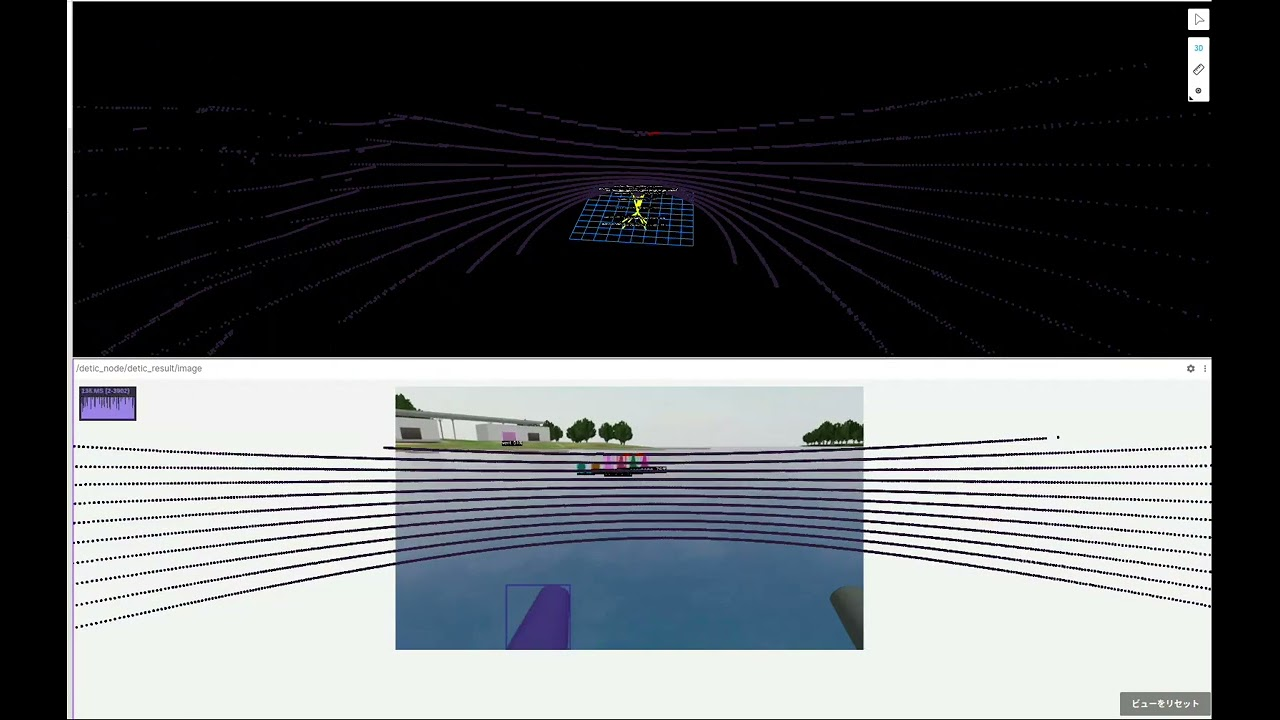
\includegraphics{figure/object_detection.jpg}
    }
  \end{center}
  \caption{Object Detection with detic and point painting.}
  \label{fig:arch_nav}
\end{figure}

The integration of Lidar and images is achieved by overlaying Detic object recognition results on point cloud data using an algorithm called point painting.

\subsection{Planning}

Path planning is divided into two components: the behavior tree, which determines the goal point, and the module, which determines the route.
The behavior tree specifies the “next goal point” based on object recognition results.
One of the issues currently discovered is the possibility of the vessel running out of control if there is an error in the object recognition results, so it is necessary to adopt a more robust algorithm in the future.
The path planner consists of a smooth path and velocity planning module using Hermite curves.
The path planner draws a smooth path that does not contact any obstacles until the goal point, and performs velocity planning in the Frenet coordinate system defined on the path.
The velocity planning module is designed to be scalable in the future, so that two independent ROS nodes can plan the velocity for each constraint condition and then compile them into a velocity plan that satisfies all the constraint conditions.

\subsection{Control}

The control of the hull is implemented with a simple PID control system, considering the hull as a Diff Drive robot.
The reason why this system was adopted is that there are not enough sensors to model the hull sway and wind, and there is a possibility that a lot of noise could get on the hull.
We adopted the simplest algorithm because we thought it would be impossible to achieve highly accurate control in any way.

\end{document}
